Consider the tachometer system shown below. 
\begin{center}
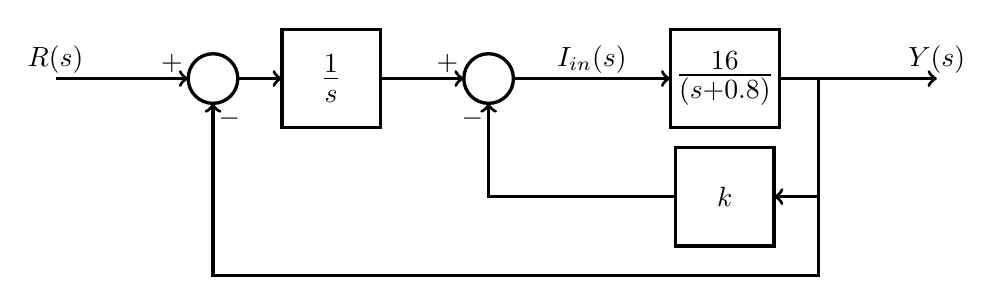
\begin{tikzpicture}[scale=1,inner sep=0pt,outer sep=0pt,very thick,
sysblock/.style={draw,rectangle,inner sep=2pt,minimum width=1.25cm,minimum height=1.25cm,very thick}]
\draw (2,0) node[draw,circle] (sum1) {$\rule{0pt}{18pt}$};
\draw (3.5,0) node[sysblock] (Kp) {\Large $\frac{1}{s}$};
\draw (5.5,0) node[draw,circle] (sum2) {$\rule{0pt}{18pt}$};
\draw (8.5,0) node[sysblock] (G) {\Large $\frac{16}{(s+0.8)}$};
\draw (8.5,-1.5) node[sysblock] (Kd) {$k$};
\draw[->] (0,0) node[above=2pt] {$R(s)$} -- (sum1.180) node[above left=2pt] {$+$};
\draw[->] (sum1.0) --  (Kp);
\draw[->] (Kp) -- (sum2.180) node[above left=2pt] {$+$};
\draw[->] (sum2.0) -- node[pos=.5,above=2pt] {$I_{in}(s)$} (G.180);
\draw[->] (G.0) -- ++(2,0) node[above=2pt] {$Y(s)$};
\draw[->] (G.0) ++(0.5,0) |- (Kd.0);
\draw[->] (Kd.180) -| (sum2.-90) node[below left=2pt] {$-$};
\draw[->] (G.0) ++(0.5,0) -- ++(0,-2.5) -| (sum1.-90) node[below right=2pt] {$-$};
\end{tikzpicture}
\end{center}
\begin{enumerate}[(a)]
\item  Find the closed loop transfer function $\frac{Y(s)}{R(s)}$ and determine the value of $k$ such that the damping ratio of the poles of this transfer function  is $0.5$. 
\item  For this value of $k$, find the rise time $t_{r}$, maximum overshoot, and settling time $t_{s}$, if $R(s)$ is a unit step.
\item  For this value of $k$, plot the step response of  $\frac{Y(s)}{R(s)}$ using \textsc{Matlab} (See Lecture \FirstOrderResponseNumber, \FirstOrderResponseName
), print it,  and mark the rise time and settling time on this graph.
\end{enumerate}


